\documentclass[12pt,a4paper,onecolumn]{article}
\usepackage[utf8]{inputenc}
\usepackage[T1]{fontenc}
\usepackage[french]{babel}

% ------------------------- Color table ----------------------------------------

\usepackage{siunitx}
\usepackage{booktabs}
\usepackage{multirow}
\usepackage[table]{xcolor}
\definecolor{maroon}{cmyk}{0,0.87,0.68,0.32}
% ------------------------------------------------------------------------------

\usepackage{amscd}
\usepackage{amsthm}
\usepackage{physics}
\usepackage[left=2.2cm,right=2.2cm,top=2cm,bottom=2cm]{geometry}
\usepackage{textcomp,gensymb} %pour le °C, et textcomp pour éviter les warning
\usepackage{graphicx} %pour les images
\usepackage{caption}
\usepackage{subcaption}
\usepackage[colorlinks=true,
	breaklinks=true,
	citecolor=blue,
	linkcolor=blue,
	urlcolor=blue]{hyperref} % pour insérer des liens
\usepackage{epstopdf} %converting to PDF
\usepackage[export]{adjustbox} %for large figures

\usepackage{array}
\usepackage{dsfont}% indicatrice : \mathds{1}


% -------------------------- Mathematics ---------------------------------------
\graphicspath{{images/}} % For the images path
% ------------------------------------------------------------------------------

% -------------------------- Mathematics ---------------------------------------
\usepackage{mathrsfs, amsmath, amsfonts, amssymb}
\usepackage{bm}
\usepackage{mathtools}
\usepackage[Symbol]{upgreek} % For pi \uppi different from /pi
\newcommand{\R}{\mathbb{R}} % For Real space


% -------------------------- Footers / header ----------------------------------
\usepackage{fancyhdr}
\pagestyle{fancy}
% ------------------------------------------------------------------------------


% -------------------------- Code format ---------------------------------------
\usepackage[numbered,framed]{matlab-prettifier}
\lstset{
	style              = Matlab-editor,
	basicstyle         = \mlttfamily,
	escapechar         = '',
	mlshowsectionrules = true,
}
% ------------------------------------------------------------------------------

% ------------------------- Blbiographie --------------------------------------
\usepackage[backend=biber, style=ieee]{biblatex}
\usepackage{csquotes} %for biblatex warning
\addbibresource{biblio.bib}
% ------------------------------------------------------------------------------

%\setcounter{tocdepth}{4} %Count paragraph
%\setcounter{secnumdepth}{4} %Count paragraph
\usepackage{float}

\usepackage{graphicx} % for graphicspath

\usepackage{array,tabularx}
\newcolumntype{L}[1]{>{\raggedright\let\newline\\\arraybackslash\hspace{0pt}}m{#1}}
\newcolumntype{C}[1]{>{\centering\let\newline\\\arraybackslash\hspace{0pt}}m{#1}}
\newcolumntype{R}[1]{>{\raggedleft\let\newline\\\arraybackslash\hspace{0pt}}m{#1}}

% \setcounter{section}{5} % to start counting section to 6

% Independent sign
\newcommand{\indep}{\ensuremath{\,\bot\!\!\!\bot\,}} %% The symbol for independent

% Alpha / Numbers for sections
\renewcommand{\thesubsubsection}{\arabic{section}.\arabic{subsection}.\alph{subsubsection})}

% % Norm
% \newcommand{\norm}[1]{\left\lVert#1\right\rVert}


% ------------------------ General informations --------------------------------
\title{Unsupervised Learning}
\author{Vincent Matthys}
\graphicspath{{images/}}
% ------------------------------------------------------------------------------

\begin{document}
\begin{tabularx}{0.8\textwidth}{@{} l X r @{} }
	{\textsc{Master MVA}}          &  & \textsc{Project 1} \\
	\textsc{Unsupervised learning} &  & {Vincent Matthys}  \\
\end{tabularx}
\vspace{1.5cm}
\begin{center}
	\rule[11pt]{5cm}{0.5pt}

	\textbf{\LARGE \textsc{Project 1: Face Completion and Movie Recommendation Challenge}}
	\vspace{0.5cm}\\
	Vincent Matthys\\
	vincent.matthys@ens-paris-saclay.fr\\
	\rule{5cm}{0.5pt}
	\vspace{1.5cm}
\end{center}

This is the first project of the course \textit{Unsupervised learning} given by René Vidal. The following assignment was related to \S 3.1 of his textbook~\cite{vidal2016principal}. Please note that the derivation presented here are extracted from his book.

\section{Low Rank Matrix Completion}

The implementation can be found in the \textit{Implementations} part of the jupyter notebook.

\section{Face completion}

In this section, we try to complete an assumed low rank matrix, X, composed of images (168x192 pixels) of the face of individual 1, a.k.a. \textit{YaleB01} of the Yale B dataset, under different illumination conditions. As we will verify, those images lie near a lower dimensional subspace. Our goal here is to complete the matrix of images X sampled uniformly at random, with the lower rank possible, and so find the matrix A minimizing :

\begin{equation}
	\begin{aligned}
		 & \underset{A}{\text{minimize}}
		 &                               & rank(A)                                           \\
		 & \text{subject to}
		 &                               & \mathcal{P}_{\Omega}(A) = \mathcal{P}_{\Omega}(X)
	\end{aligned}
	\label{eq_hard}
\end{equation}

where \(P_{\Omega}(X)\) denotes the observed entries.

The problem~\eqref{eq_hard} can be relaxed as explained in the textbook~\cite{vidal2016principal} to this one :

\begin{equation}
	\begin{aligned}
		 & \underset{A}{\text{minimize}}
		 &                               & \tau \lVert A \rVert_* + \frac{1}{2}\lVert A \rVert_F^2 \\
		 & \text{subject to}
		 &                               & \mathcal{P}_{\Omega}(A) = \mathcal{P}_{\Omega}(X)
	\end{aligned}
	\label{eq_hard}
\end{equation}

And the solution can be computed iteratively by finding the saddle point of the Lagrangien \(\mathcal{L}\) :
\begin{equation}
	\left\{
	\begin{split}
		A_{k+1} &= \underset{A}{\text{argmin}\,\mathcal{L}(A, Z_k)}\\
		Z_{k+1} &= Z_k + \beta \frac{\partial\mathcal{L}}{\partial Z}\left(A_{k+1}, Z_k)\right)
	\end{split}
	\label{eq_algo}
	\right.
\end{equation}
where \(Z\) is the lagrangian multiplier associated with the constraint. Finaly, the algorithm of low rank matrix completion by proximal gradient implemented before is simply computing the A for the saddle node.

The faces completion is shown in figure~\ref{fig_faces} for different percentage of missing entries and different \(\tau\). A quasi perfect completion, except in shadow areas next to the nose, is reached until \(70~\%\) of missing entries, with a minimal MSE for \(\tau = 6\times10^5\) of \(96.5\). The results are comparable with the ones in the book, figure 3.2. We didn't reproduce the behaviour in large \(\tau\), as our algorithm, as implemented, didn't converge for values of \(\tau\) to high. The same append for values of \(\tau\) lower than 50000.

\begin{figure}[H]
	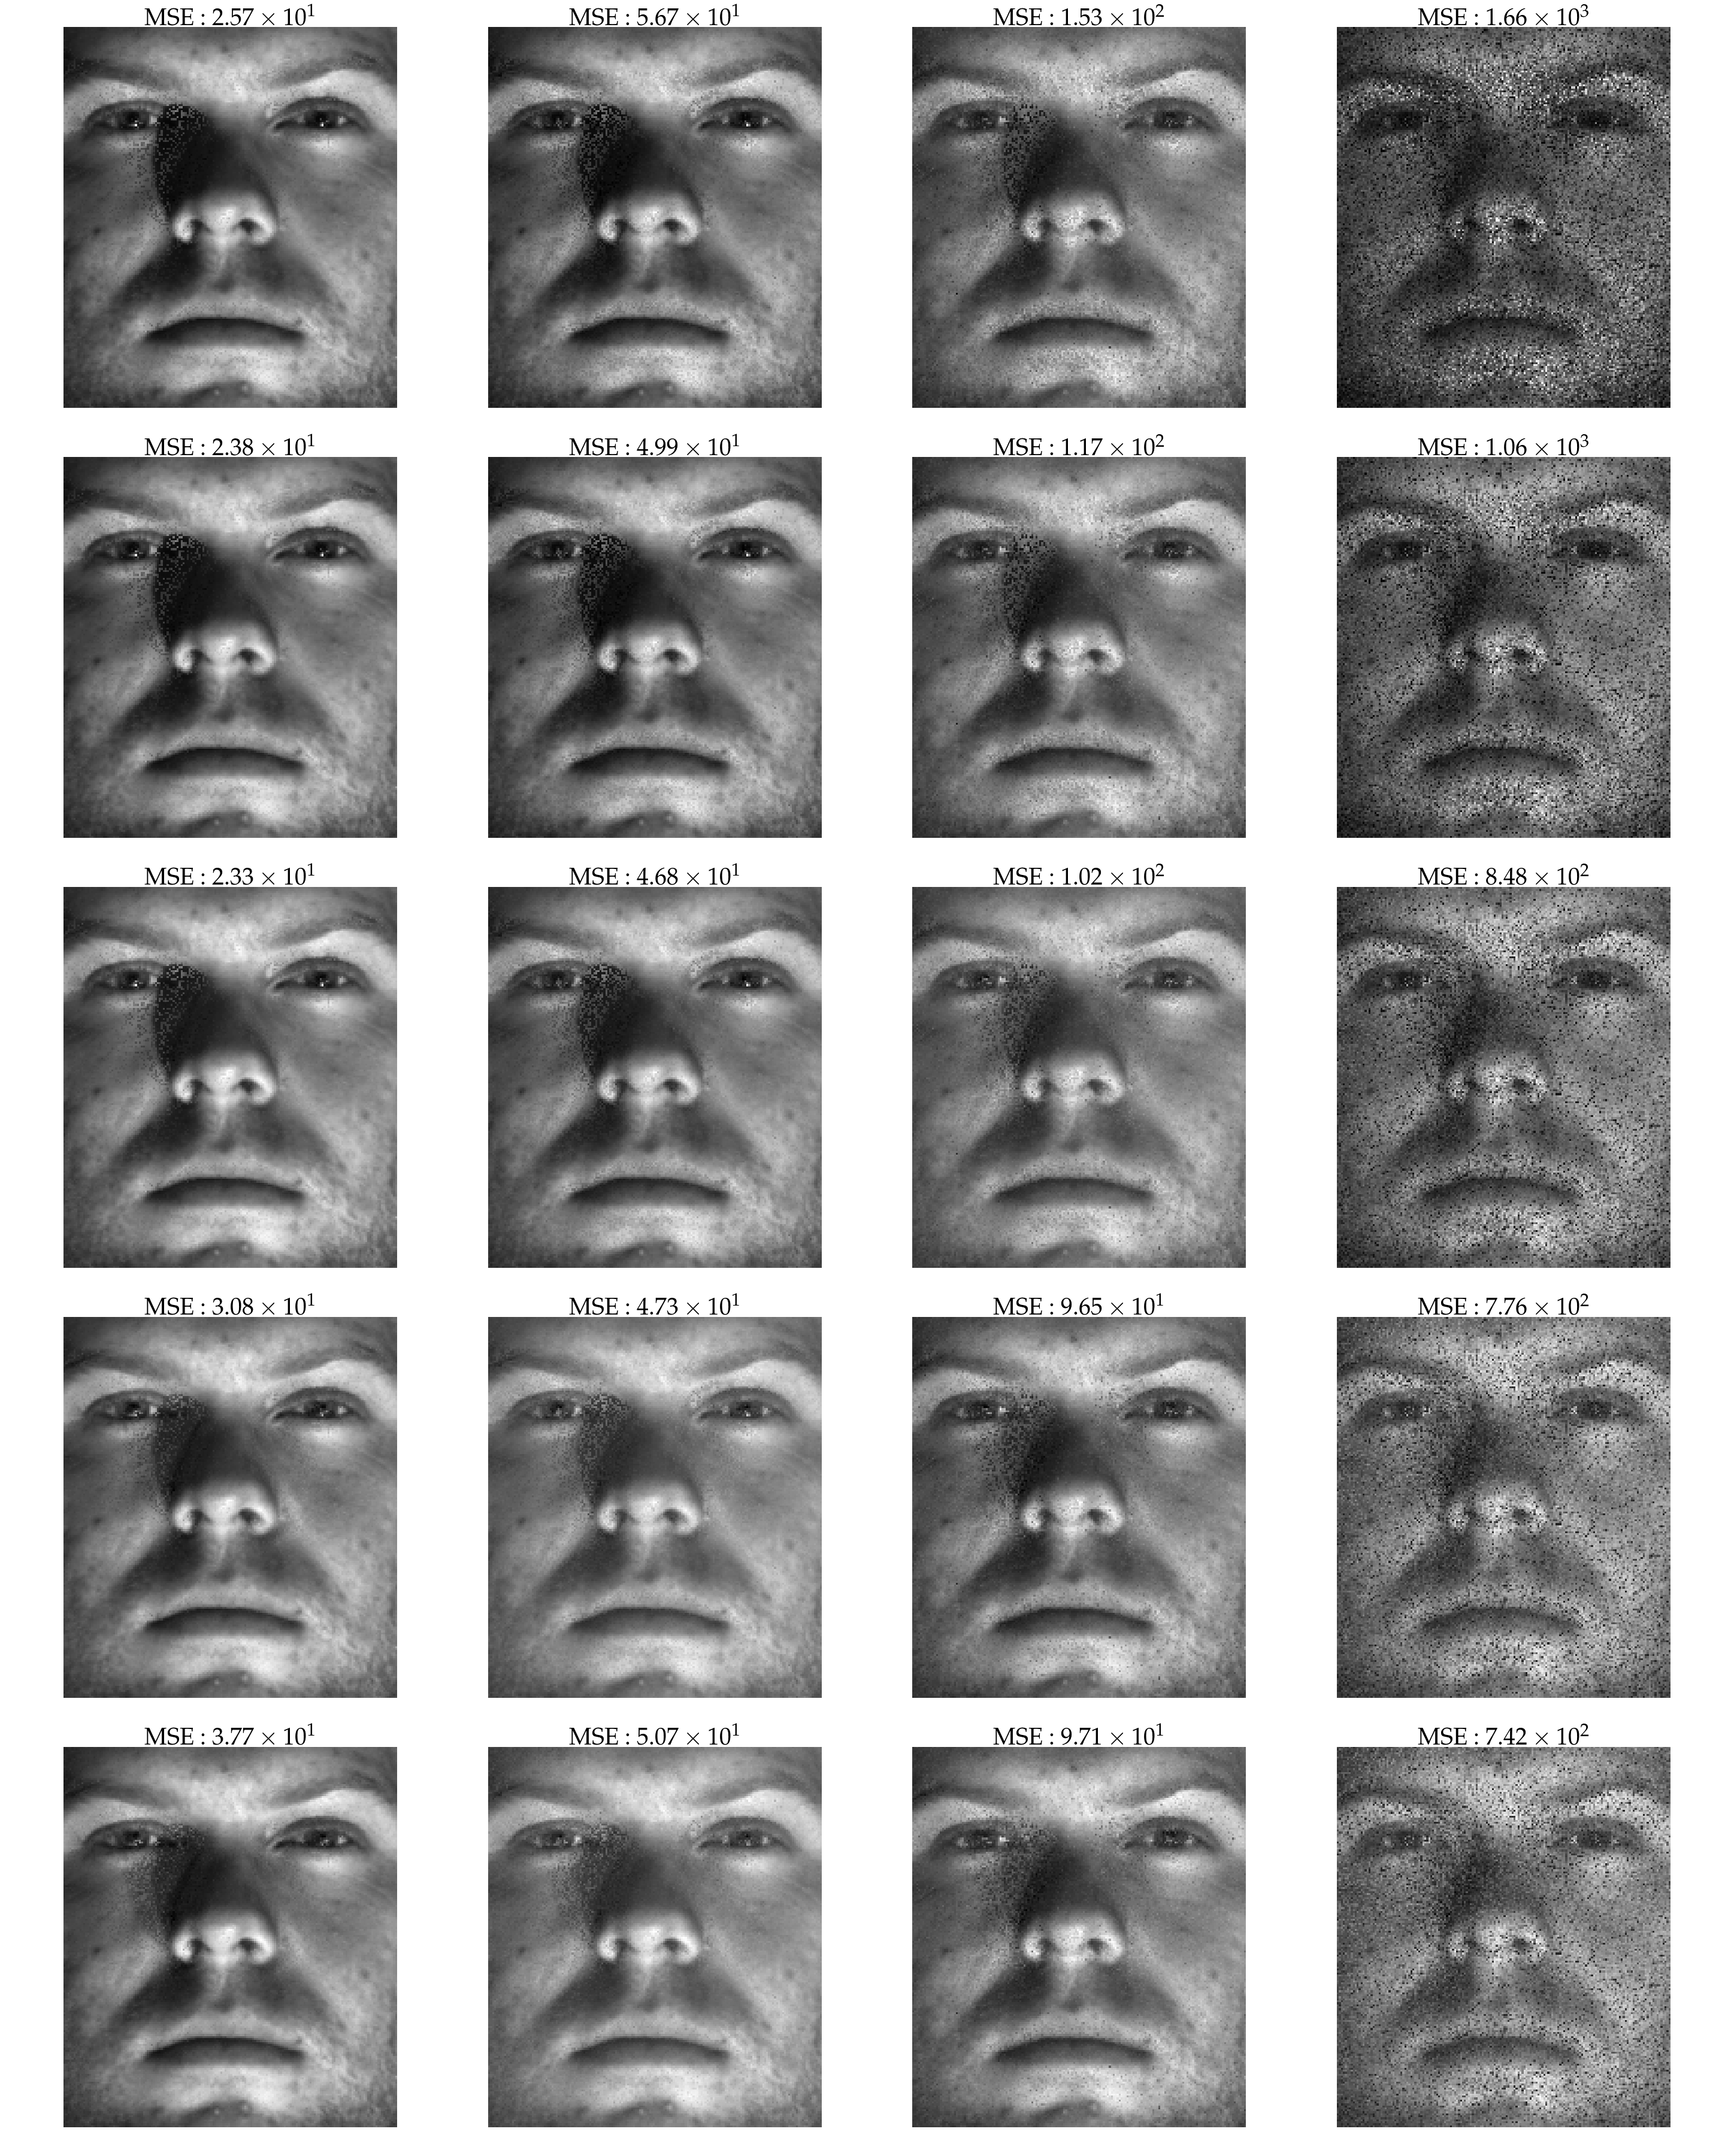
\includegraphics[width = 1.0\textwidth]{2_bis.png}
	\caption{Faces completion with low ranl matrix completion algorithm. Lines 1 to 5 : \(\tau = [1, 2, 4, 6, 8] \times 10^{5}\). Columns 1 to 5 : \(\%(\text{missing entries}) = [30, 50, 70, 90]\times \%\)}
	\label{fig_faces}
\end{figure}

In figure~\ref{fig_curve} is presented the evolution of MSE in function of \(\tau\). It shows that the larger tau, the lower is the MSE, and better is the completion. It's a common result, as the relaxation of the problem is closer to the true one when \(\tau\) is bigger.

\begin{figure}[H]
	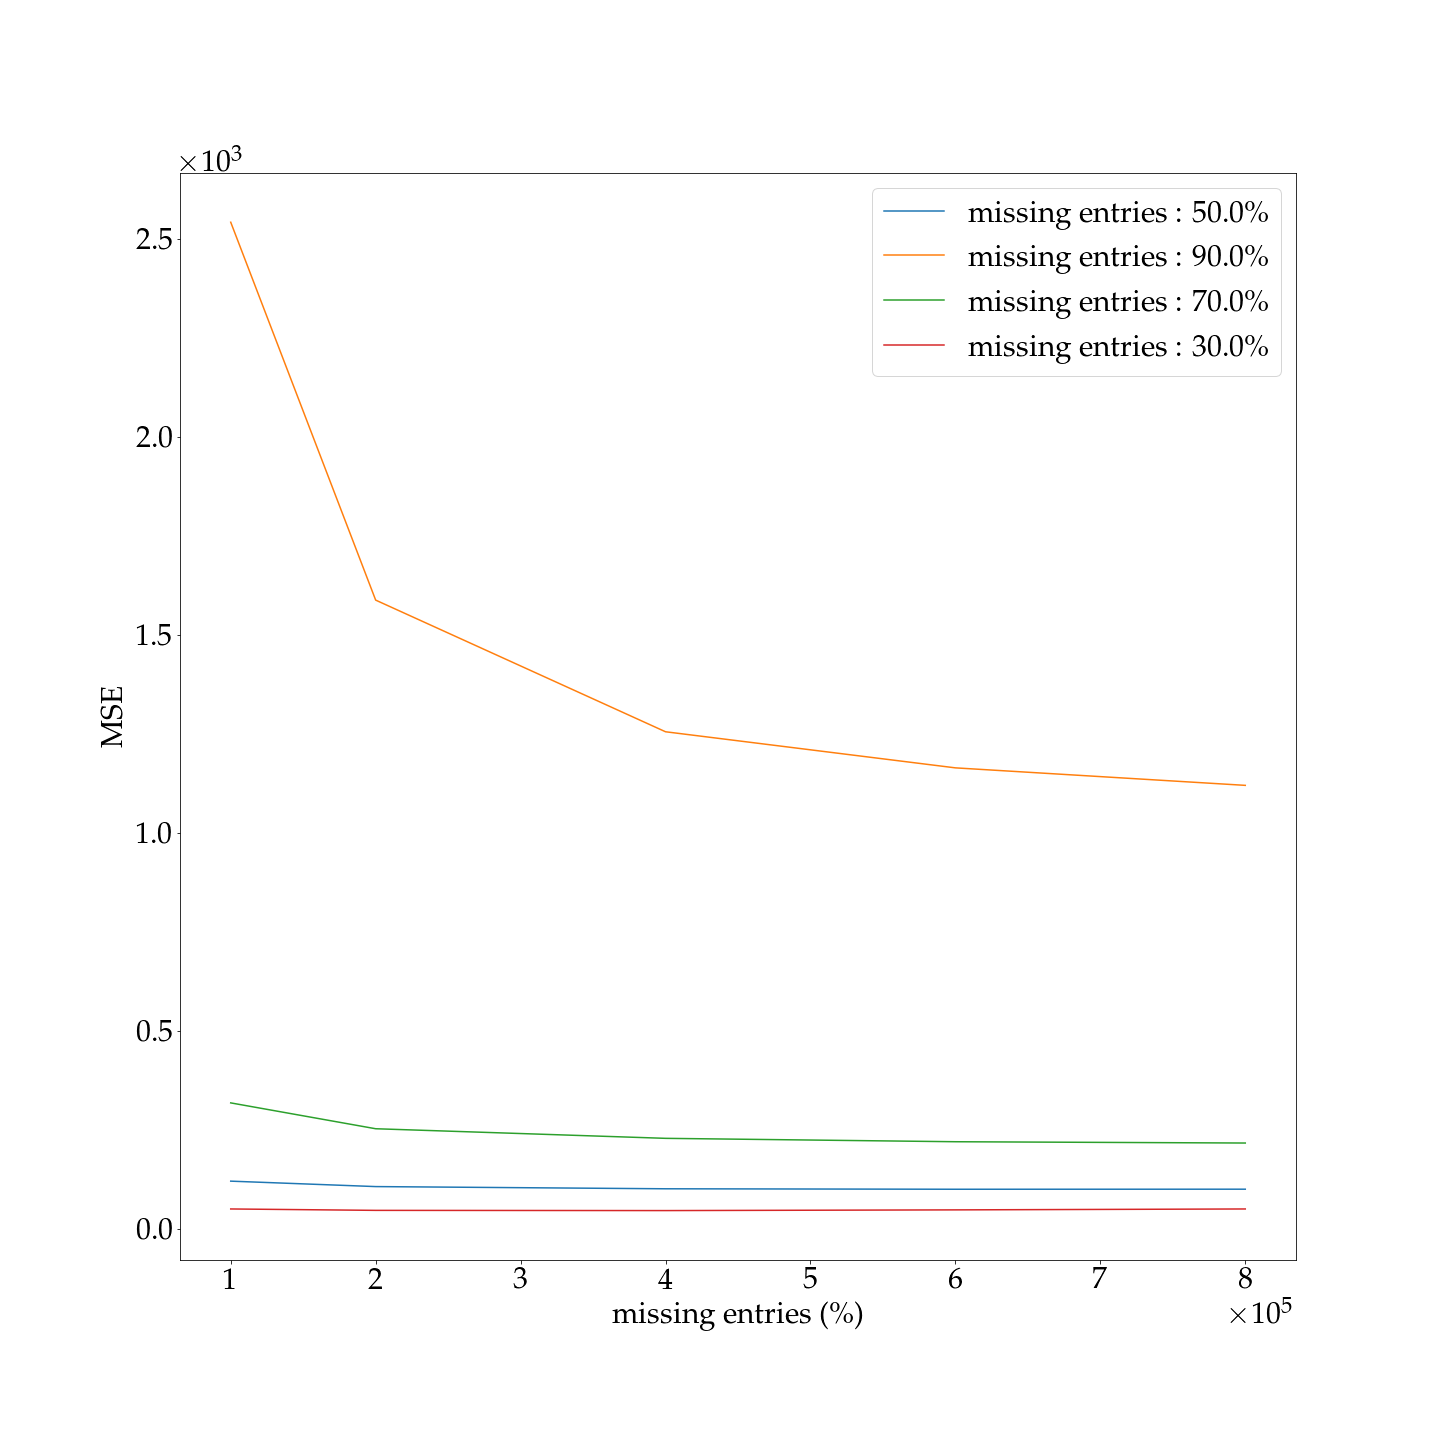
\includegraphics[width = 1.0\textwidth]{2_curve.png}
	\caption{MSE function of \(\tau\) for the faces represented in \ref{fig_faces}}
	\label{fig_curve}
\end{figure}

\section{Movie recommandation Grand Challenge}

For the movie recommandation Grand Challenge, the results are shown in table~\ref{tab_moovie}. All the results were computed for \(\beta = 2\), and for \(10~\%\) of training data. It is not surprising to see that the completion works better (because we have a lower MSE) for the single-genre ratings, as the rank should be lower. Moreover, we noticed a high sensibility for the beta parameter, which didn't allow us to do a real grid search. The case \(\beta = 2\) worked just fine.

\begin{table}
	\centering
	\begin{tabular}{r | r | r}
		\hline
		Genres            & \(\tau\)     & MSE   \\\hline
		Horror            & \(10^5\)     & 0.156 \\\hline
		Romantic          & \(10^4\)     & 0.177 \\\hline
		Romantic + Horror & \(1.2~10^3\) & 0.349 \\\hline
	\end{tabular}
	\caption{MSE on the test set held out for Horror ratings, Romantic ratings, and Romantic \& Horror ratings}
	\label{tab_moovie}
\end{table}

\printbibliography
\end{document}
